% !TEX TS-program = xelatex
% !TEX encoding = UTF-8 Unicode
% !Mode:: "TeX:UTF-8"

\documentclass{resume}
\usepackage{zh_CN-Adobefonts_external} % Simplified Chinese Support using external fonts (./fonts/zh_CN-Adobe/)
% \usepackage{NotoSansSC_external}
\usepackage{NotoSerifCJKsc_external}
% \usepackage{zh_CN-Adobefonts_internal} % Simplified Chinese Support using system fonts
\usepackage{linespacing_fix} % disable extra space before next section
\usepackage{cite}
\usepackage{graphicx}
\usepackage{tabu}
\usepackage{multirow}
\usepackage{progressbar}

\begin{document}
\pagenumbering{gobble} % suppress displaying page number

\begin{center}
\Huge{个~~~人~~~简~~~历}
\end{center}
\\
\Large{
  \begin{tabu}{ c l l }
   \multirow{5}{1in}{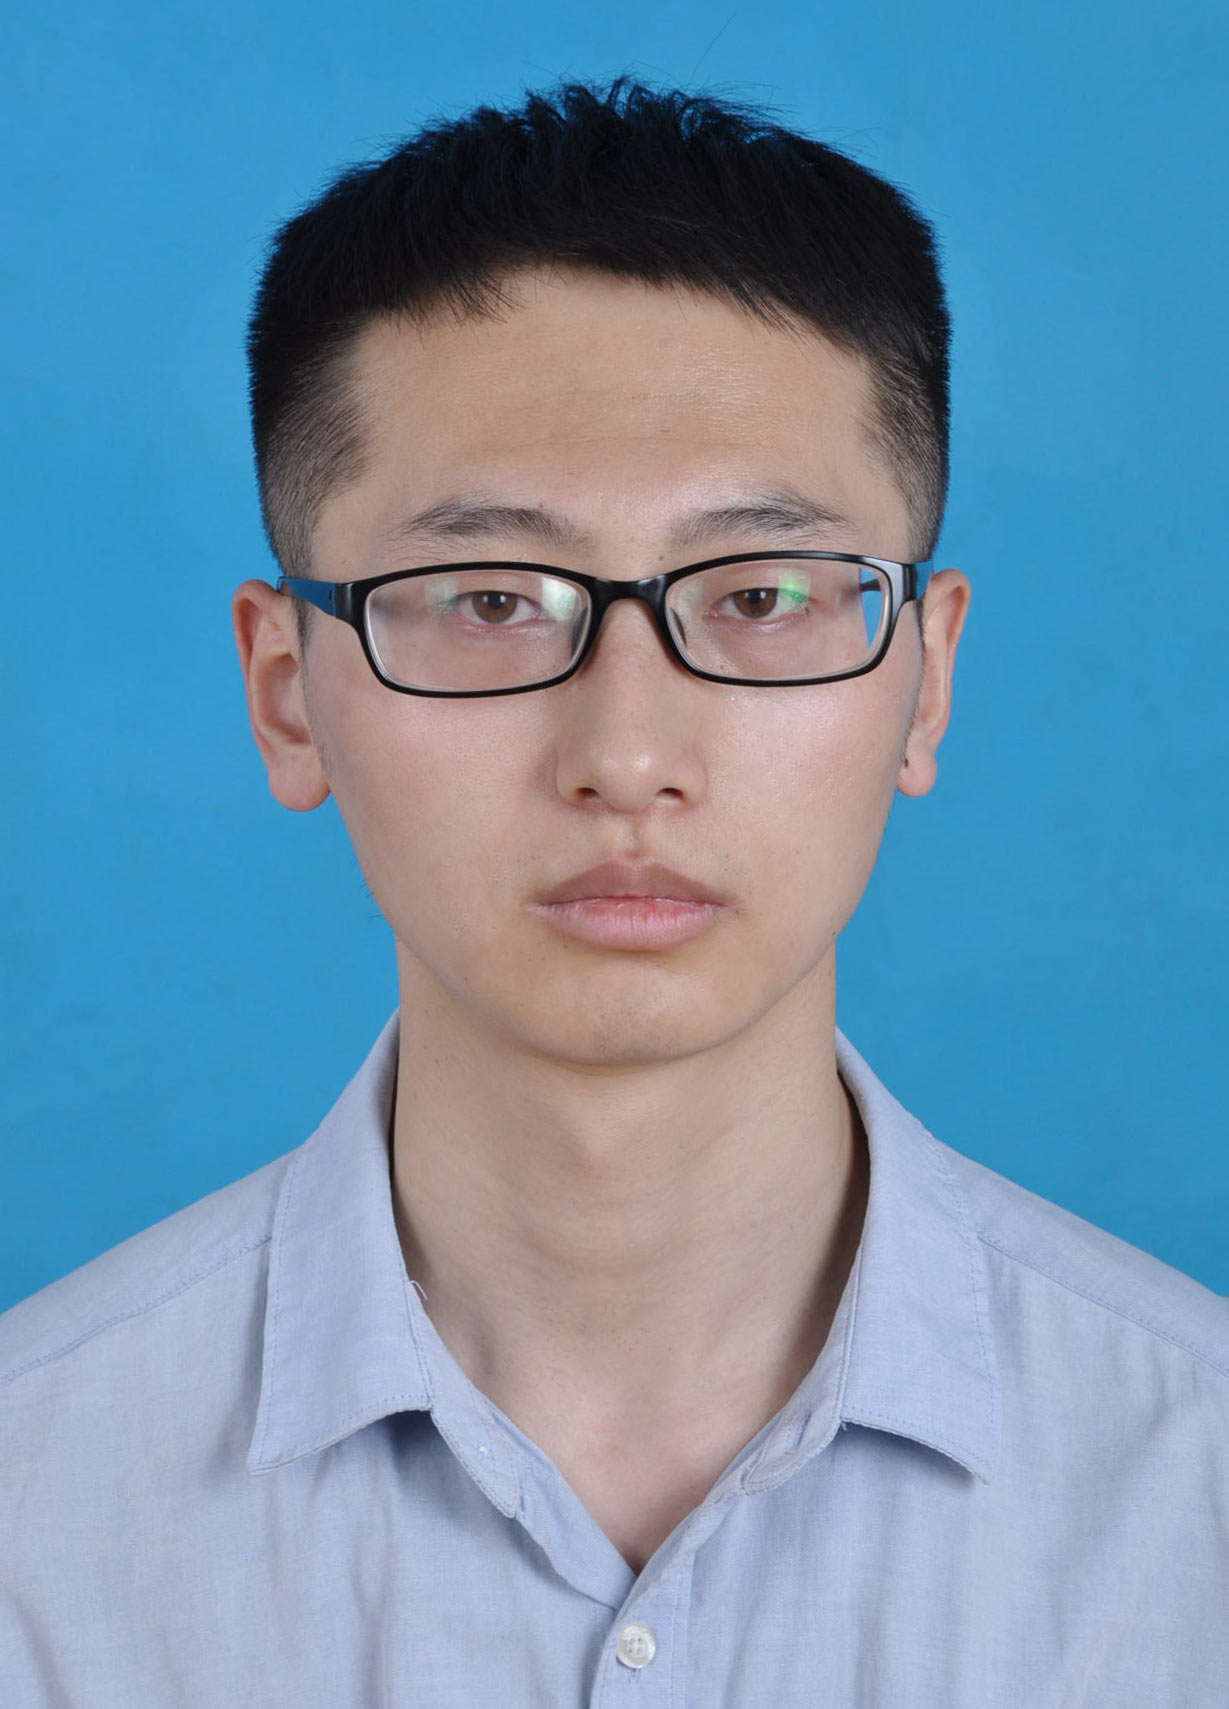
\includegraphics[width=0.88in]{avatar}} &
   \scshape{李高阳} &  \\
    & 性别:男 & 民族:汉 \\
    & 电话:(+86) 15682897374 & 生日:1991-09 \\
    & 邮箱:li.gaoyang@foxmail.com & 微信:sandbox\_ligy\\
    & 地址:甘肃省兰州市天水南路222号 \hspace{40} & %籍贯:甘肃宁县
  \end{tabu}
}

\section{教育经历}
% \textbf{兰州大学}
\datedsubsection{\textbf{兰州大学\ 硕博连读与中科院兰州近物所联合培养博士}}{2013 -- 2019}
\textit{专业:理论物理}\\
\textit{方向:强关联量子系统的数值求解}
\datedsubsection{\textbf{兰州大学\ 本科}}{2009 --  2013}
\textit{专业:物理学国家基地班\ \ 理论物理}

\section{获奖情况}
\datedline{\textit{国家励志奖学金}}{2010 -- 2011}
% \datedline{其他奖项}{2015}

\section{项目经验}
\begin{itemize}%[parsep=0.5ex]
\item \textbf{基于C++实现了全密度矩阵数值重整化群算法}\\
独立完成了程序的编写,其中涉及矩阵乘法、稠密矩阵对角化等矩阵向量操作。实现中调用了Intel MKL库,并作了单节点OpenMP并行优化。该程序已可以用来求解一些量子杂质问题,部分研究成果已整理成学术论文,正在准备发表。
\item \textbf{基于FORTRAN实现了模拟退火算法}\\
针对一个有8个自变量的函数最小值问题,调研并实现了模拟退火算法,在变分求解Rabi模型的应用中达到了较好的结果。
\item \textbf{能高效使用Shell语言,并熟悉Linux编程环境,Python等.}
\end{itemize}

\section{其他技能}
% increase linespacing [parsep=0.5ex]
\begin{itemize}%[parsep=0.5ex]
\item 英语六级467
\item 平常编写代码要求尽量高效、美观,并用git管理代码
\item 对新知识有较高的学习热情,并能投入精力解决问题
\item 了解精确对角化、密度矩阵重整化群、蒙特卡罗、级联运动方程等数值计算方法
% \item 喜欢打羽毛球
\end{itemize}

\section{个人主页}
\rm{https://github.com/GoldenRaven}

%% \section{求职意向}
%% \begin{itemize}%[parsep=0.5ex]
%% \item 算法设计与实现、机器学习相关职位
%% \end{itemize}

%% Reference
% \newpage
% \bibliographystyle{IEEETran} \bibliography{mycite}
\end{document}
